\section{Introduction}
\label{sec:intro}

This paper addresses the problem of automatically building $3$D mesh models of plant leaves using inexpensive time-of-flight RGB-D sensors.  Plant researchers, seeking to understand genetic underpinnings of plant growth [REF] and seeking to develop new varieties [REF], need automated ways to non-invasively measure plant phenotypes including growth, leaf distributions, orientations, photosynthesis and productivity [REF].  An important step in estimating all of these properties is obtaining $3$D shape and pose for all the plant leafs.  Plants cannot be moved or disturbed in limited-space growth chambers making it impractical to use scanning lasers for shape modeling.  Instead our concept is to mount close-range time-of-flight RGB-D sensors in the chambers, acquire color, IR-reflectance and range data, and estimate leaf shape through building 3D mesh models of the leafs.

While time-of-flight RGB-D sensors are small, inexpensive and provide dense 3D surface sampling of objects, they pose a challenge to surface modeling of small objects due to large depth noise.  This pixel-depth noise is significantly larger than the surface features we hope to capture, and can be on the order of the leaf size.  The goal of this paper is to cut through this noise to obtain high fidelity surface models of leaves and small objects.  


\begin{figure}
\begin{center}
\begin{tabular}{ c c }
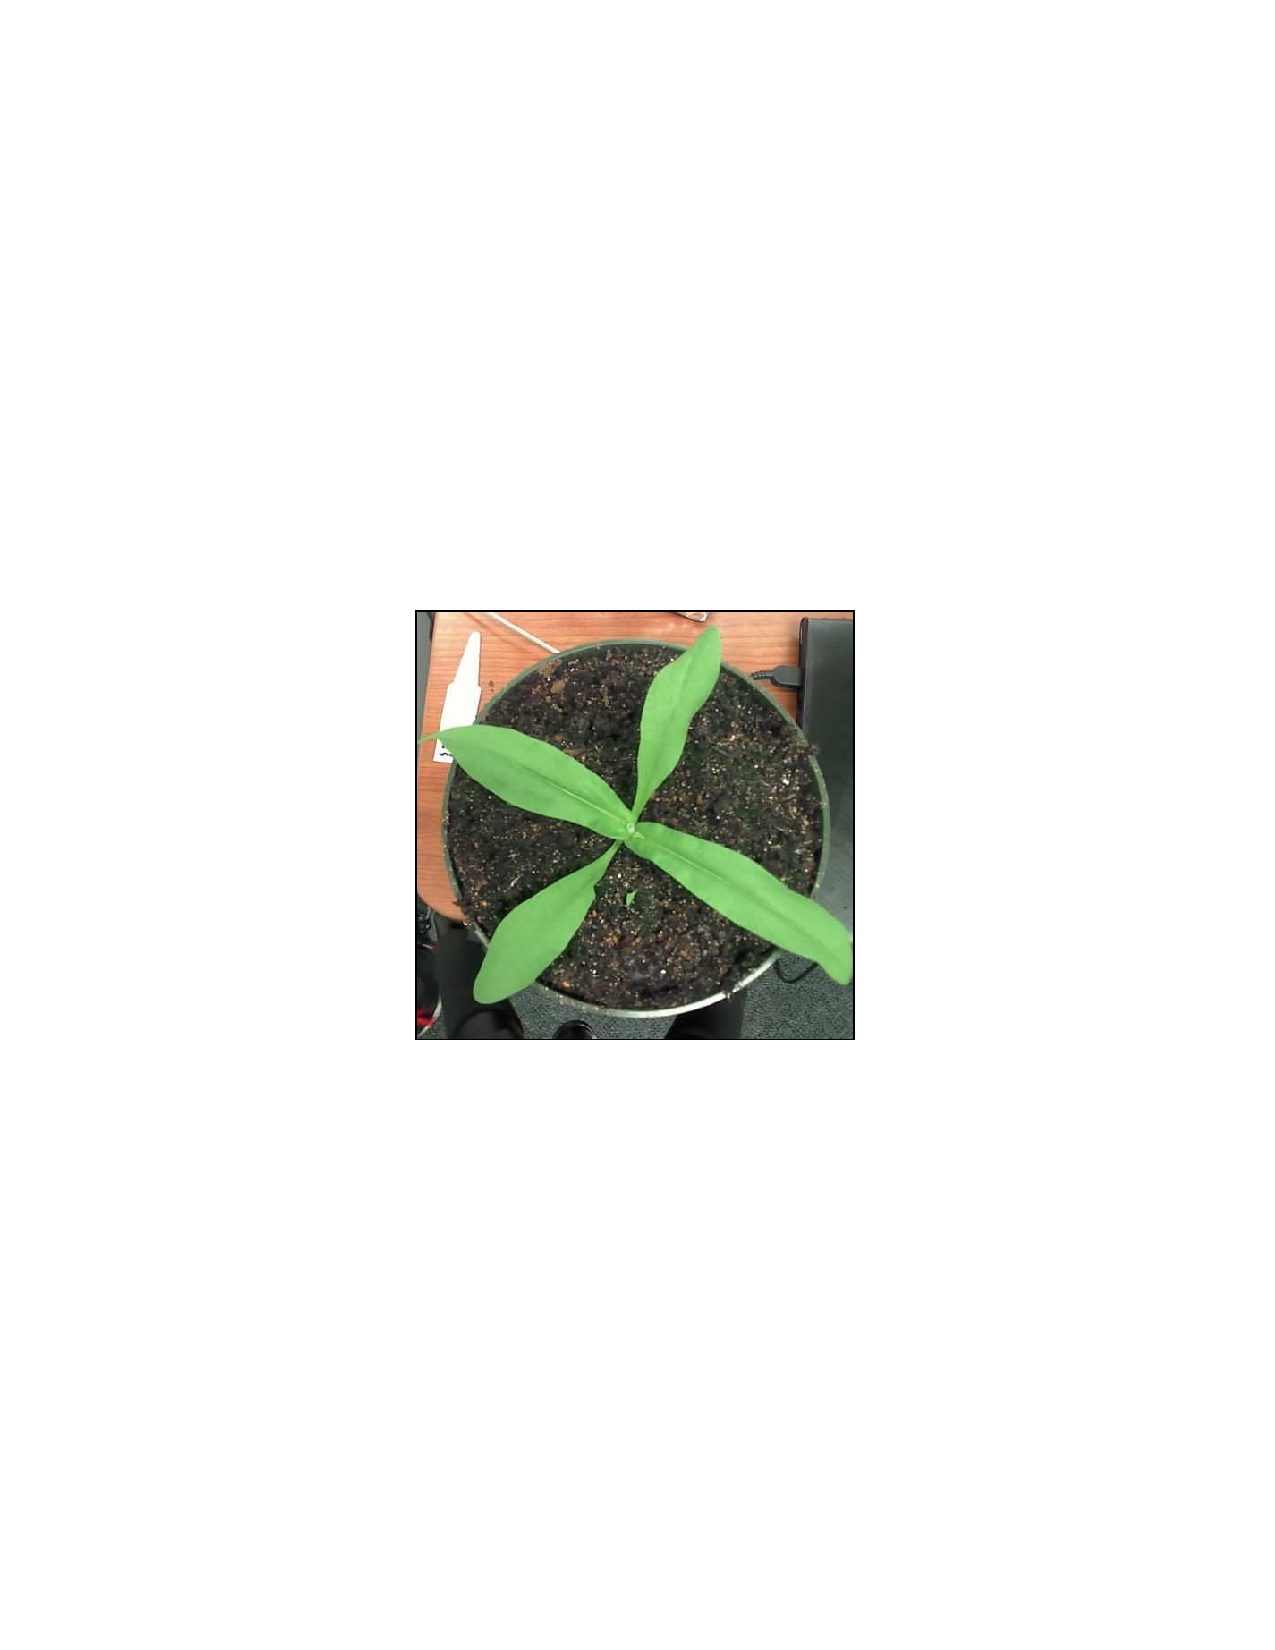
\includegraphics[trim=200 280 200 280,clip,width=0.4\linewidth]{Figures/plant1-rgb} &
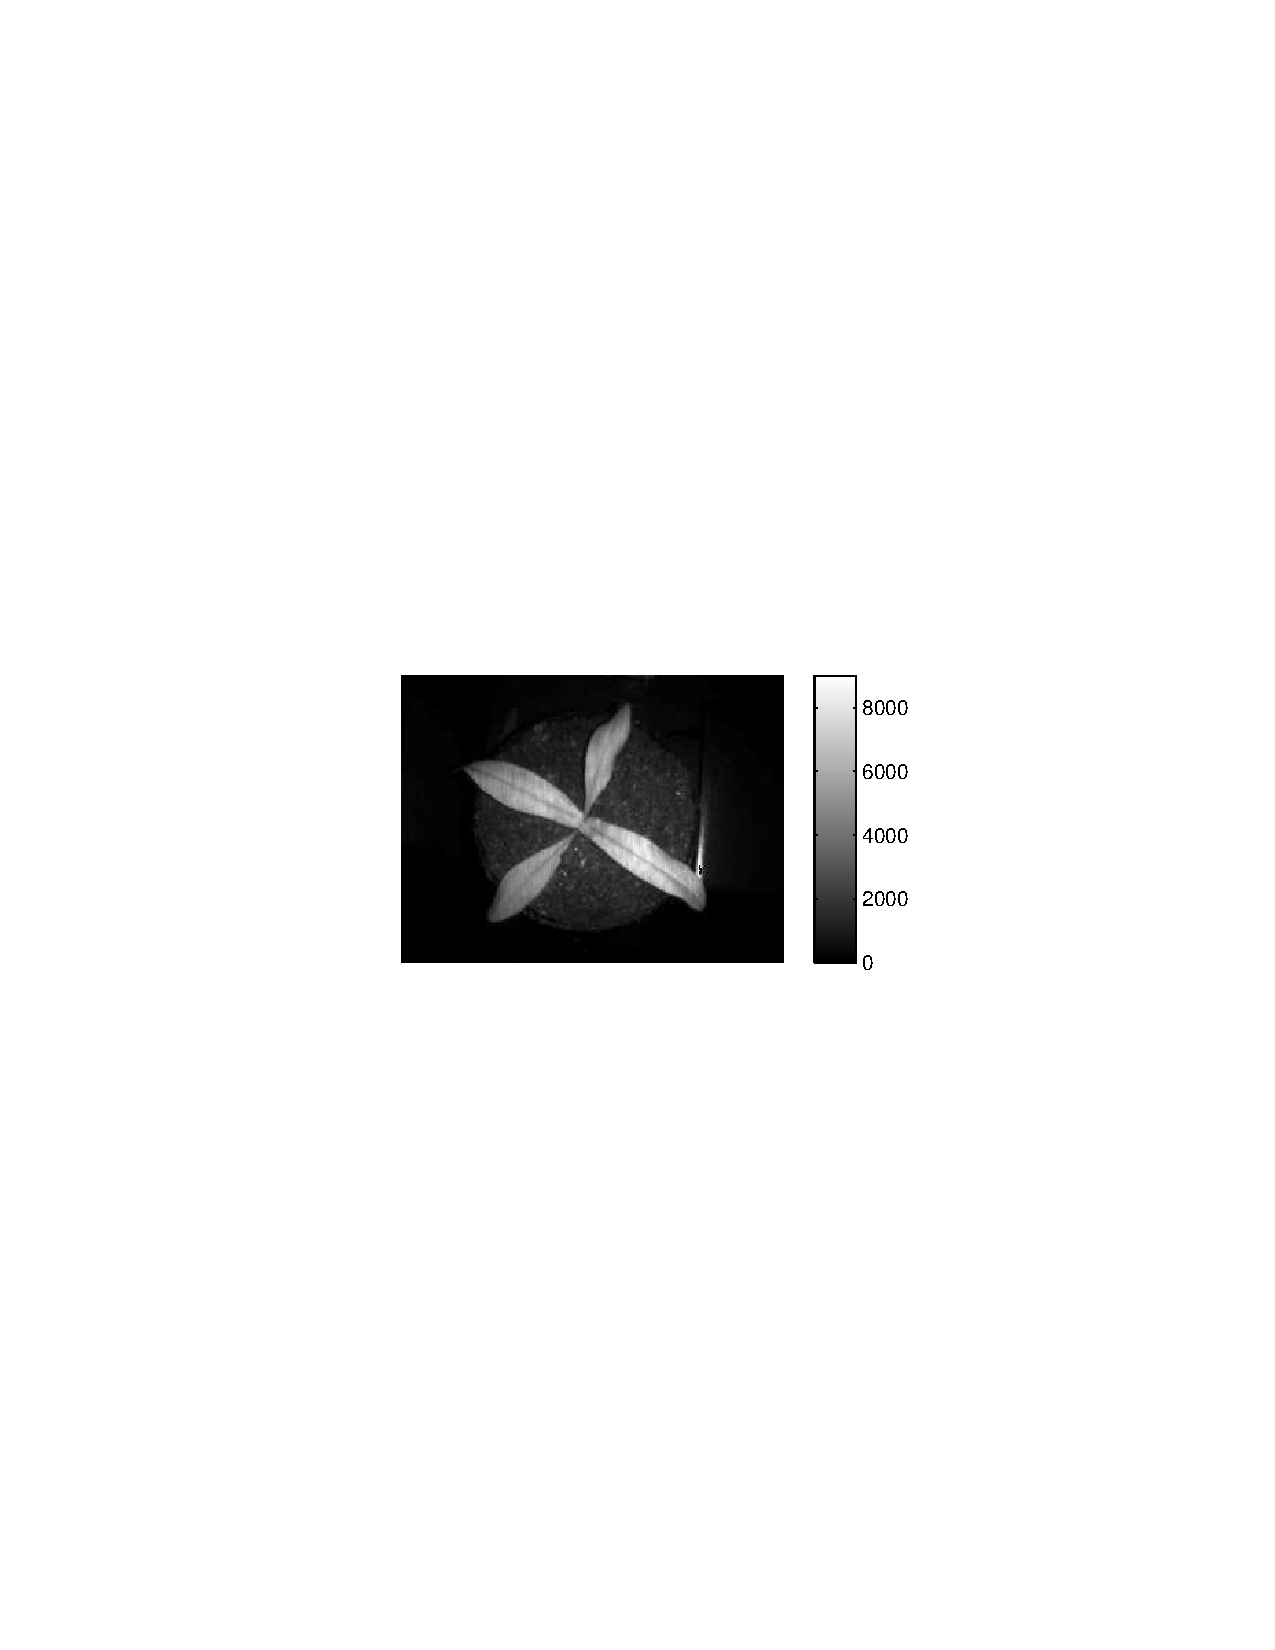
\includegraphics[trim=220 270 160 280,clip,width=0.4\linewidth]{Figures/plant1-ir} \\
($a$) & ($b$) \\
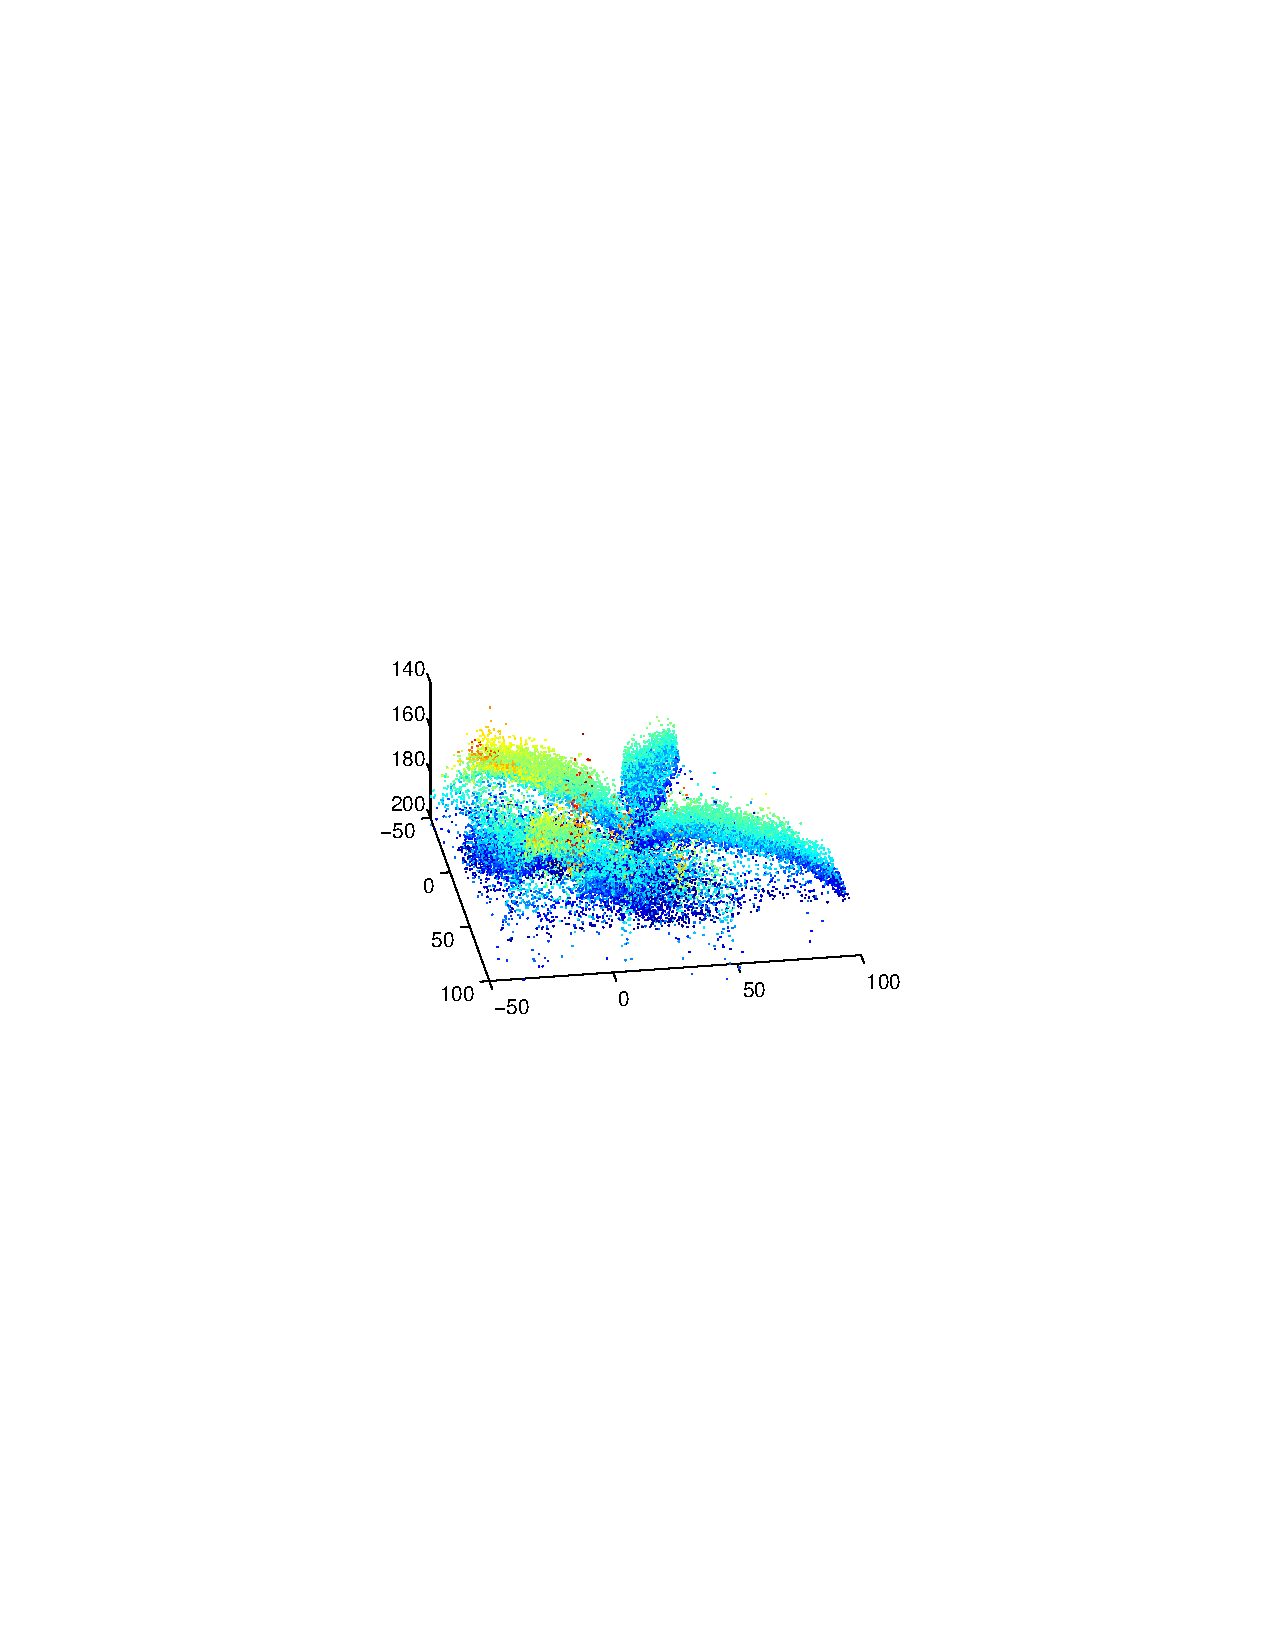
\includegraphics[trim=180 270 180 280,clip,width=0.4\linewidth]{Figures/plant1-3D-single} &
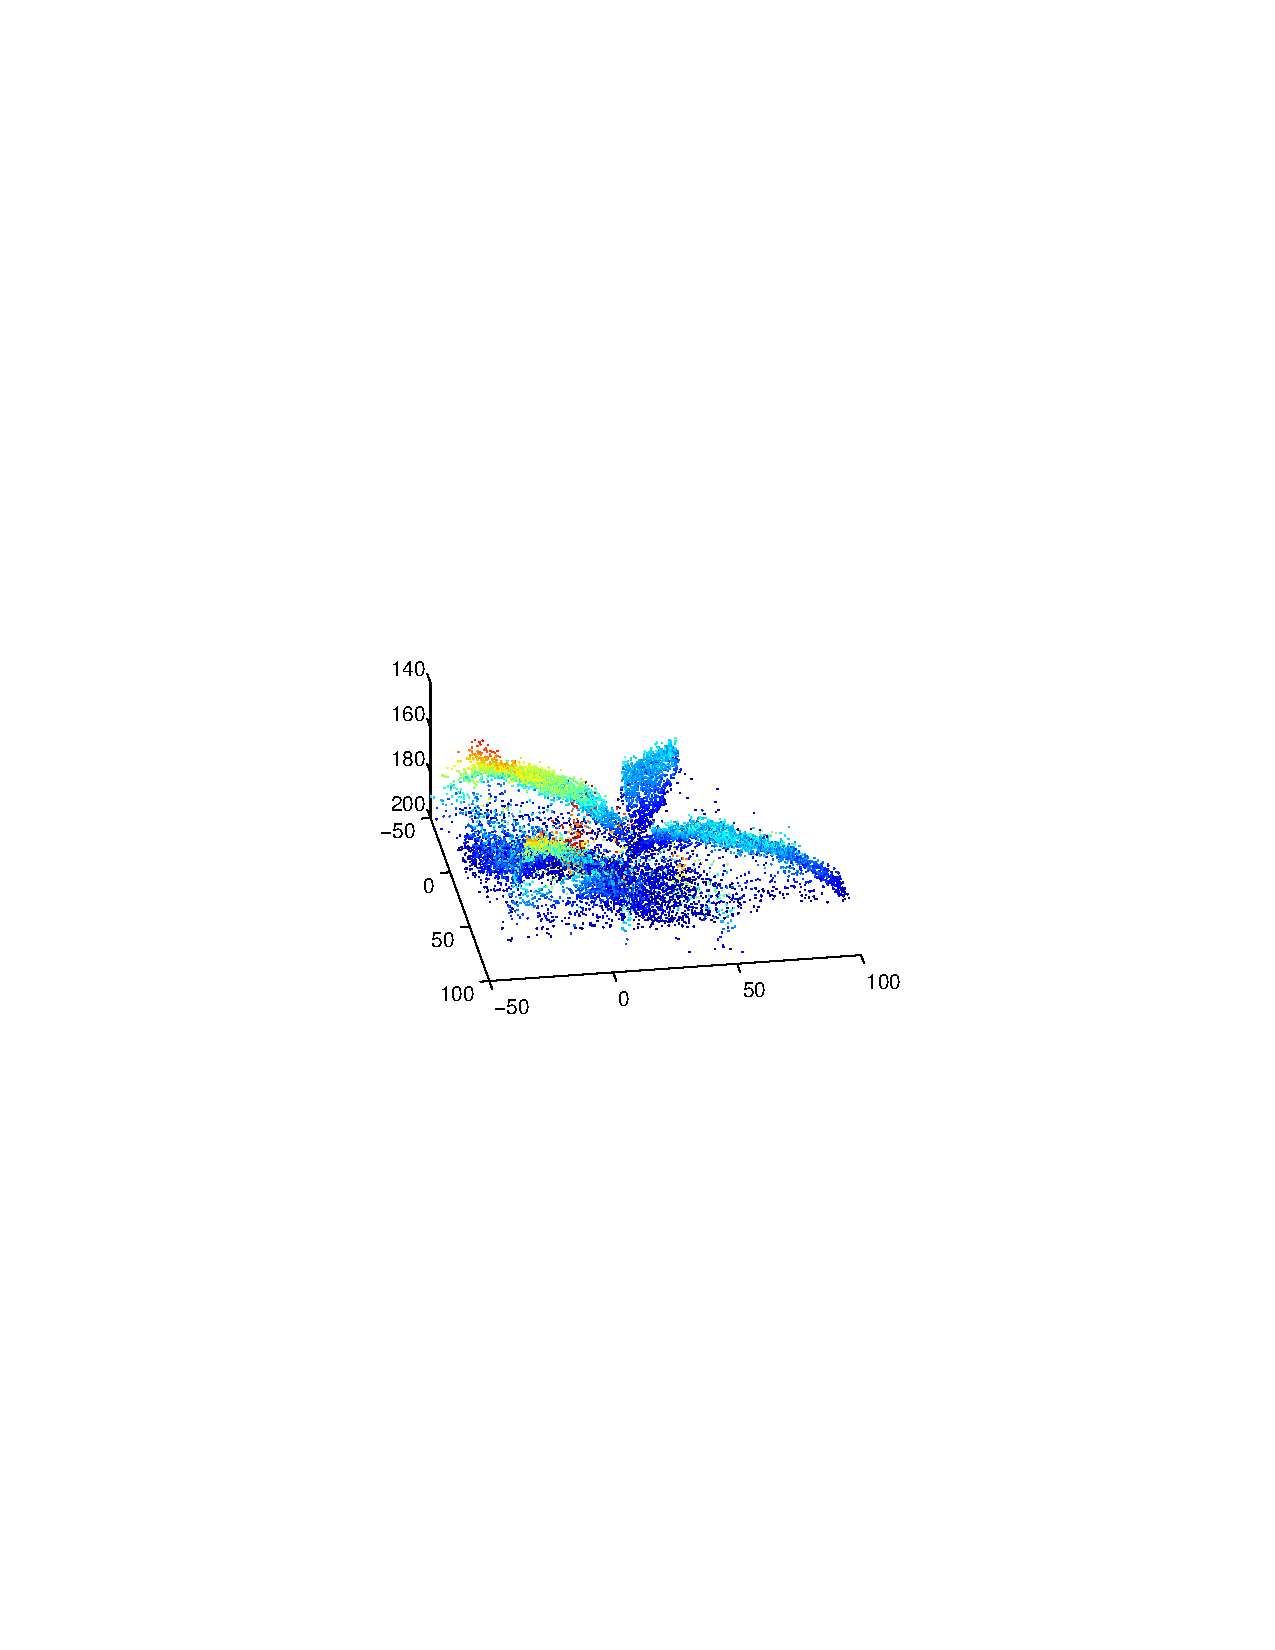
\includegraphics[trim=180 270 180 280,clip,width=0.4\linewidth]{Figures/plant1-3D-average} \\
($c$) & ($d$) \\
\end{tabular}
\end{center}
\caption{Illustration of sensor data.  ($a$) Portion of color image. ($b$) IR reflectance image with reflectance values. ($c$) Portion of a single depth image surrounding plant projected into $3$D showing significant depth noise. ($d$) Average of 60 depth images projected into $3$D, with $\sigma_S$ being the dominant source of noise.  Units of $3$D plots are mm.  The goal of this paper is to combine these data elements into }
\label{fig:plantnoise}
\end{figure}



Mesh fitting to $3$D point clouds and depth maps has had a number of objectives.  A mesh provides a surface topology and geometry to a point cloud~\cite{Sienz2000,Yeh2011}.  This enables visualization and shape analysis of the target object.  A mesh can efficiently compress dense scanned data and mesh fitting methods have been developed that adhere to the underlying shape and preserve geometric features such as creases~\cite{hoppe:1994,Kobbelt:1998}.  The problem differs from these in that our depth data are far noisier and our goal is to recover the true surface rather than adhering as closely as possible to the 3D points.

Another goal for mesh fitting is to incrementally build full $3$D models of objects.  Zippered polygons~\cite{Turk1994} builds mesh models from range images and combines them discarding noisy points at the boundaries.  The method developed by Curless and Levoy~\cite{Curless:1996} populates a weighted voxel occupancy grid from the depth data and recovers the surface by triangulating an isosurface.  By raycasting this surface, new camera poses can be aligned and their depths maps contribute to and improve the voxel model.  Advantages of this method include that surface topology is automatically determined, additional data can be readily incorporated, holes can be filled when more data are collected and it incorporates directional uncertainty of range data into the models.  Recent approaches for environment modeling from RGB-D cameras such as Kinect Fusion~\cite{Izadi:2011,Newcombe:2011} build on this voxel modeling and accumulation.  For our application the sensor is fixed and there is no option for merging views from different perspectives.  Artifacts caused by discretization into voxels are significant particularly with high input noise, and the method is limited in incorporating surface smoothness priors.

The method proposed here is a new mesh generation algorithm that resolves object shape despite large noise in the range images by leveraging multiple sensor modalities.  Edge features of the high resolution color image are used to help select and constrain vertices and mesh edges.  The errors in depth are modeled along camera rays and minimized during fitting to facets.  The IR reflectance image is used as a Shape from Shading cue to influence facet surface normals.  A linear least squares solution to Laplacian smoothing is integrated into the mesh fitting for regularization with surface curvature priors, and modification is made to preserve sharp edges and creases.


